%% Commands for TeXCount
%TC:macro \cite [option:text,text]
%TC:macro \citep [option:text,text]
%TC:macro \citet [option:text,text]
%TC:envir table 0 1
%TC:envir table* 0 1
%TC:envir tabular [ignore] word
%TC:envir displaymath 0 word
%TC:envir math 0 word
%TC:envir comment 0 0
\documentclass[sigconf,authordraft]{acmart}

\usepackage{listings}
\lstset{
  basicstyle=\ttfamily\small
}

\author{Kieran John Knowles}
\affiliation{%
  \institution{Newcastle University}
  \city{Newcastle Upon Tyne}
  \country{United Kingdom}
}

%% Rights management information.  This information is sent to you
%% when you complete the rights form.  These commands have SAMPLE
%% values in them; it is your responsibility as an author to replace
%% the commands and values with those provided to you when you
%% complete the rights form.
% TODO: Copyright
\setcopyright{none}
\copyrightyear{2025}
\begin{document}

\title{Vindolanda VR}
% TODO: Video link

% TODO: Abstract
\begin{abstract}
\end{abstract}

%% The code below is generated by the tool at http://dl.acm.org/ccs.cfm.
%% Please copy and paste the code instead of the example below.
% TODO: CCS XML
\begin{CCSXML}
\end{CCSXML}

% \ccsdesc[500]{Do Not Use This Code~Generate the Correct Terms for Your Paper}
% \ccsdesc[300]{Do Not Use This Code~Generate the Correct Terms for Your Paper}
% \ccsdesc{Do Not Use This Code~Generate the Correct Terms for Your Paper}
% \ccsdesc[100]{Do Not Use This Code~Generate the Correct Terms for Your Paper}

% TODO: Keywords
\keywords{Virtual reality, History, Education}

% TODO: Teaser
% \begin{teaserfigure}
%   \includegraphics[width=\textwidth]{sampleteaser}
%   \caption{Seattle Mariners at Spring Training, 2010.}
%   \Description{Enjoying the baseball game from the third-base
%   seats. Ichiro Suzuki preparing to bat.}
%   \label{fig:teaser}
% \end{teaserfigure}

\maketitle

\section{Introduction}
% TODO: Introduction

\section{Background \& Related Work}
% TODO: Background Research}

\subsection{Historical Research}
% TODO: Historical Research}

\subsubsection{Site Visits}
% TODO: Site Visits}

\paragraph{Vindolanda}
% TODO: Vindolanda visit}
A visit to the Vindolanda museum was arranged in order to gather reference
material.

\paragraph{Hancock Museum}
% TODO: Hancock Museum visit}

Aside from the fort itself, a visit was made to the Roman exhibits at the
Hancock Museum to gather reference material for the wall and on Roman soldiers.
This included the armour shown in Figure \ref{fig:armour}, a milecastle that
would be built every Roman mile (~1.5km) \cite[p.1027]{smith_new_1851} shown in
Figure \ref{fig:milecastle}, and a turret, two of which would be built between
each milecastle shown in Figure \ref{fig:turret}.

\begin{figure}[h]
  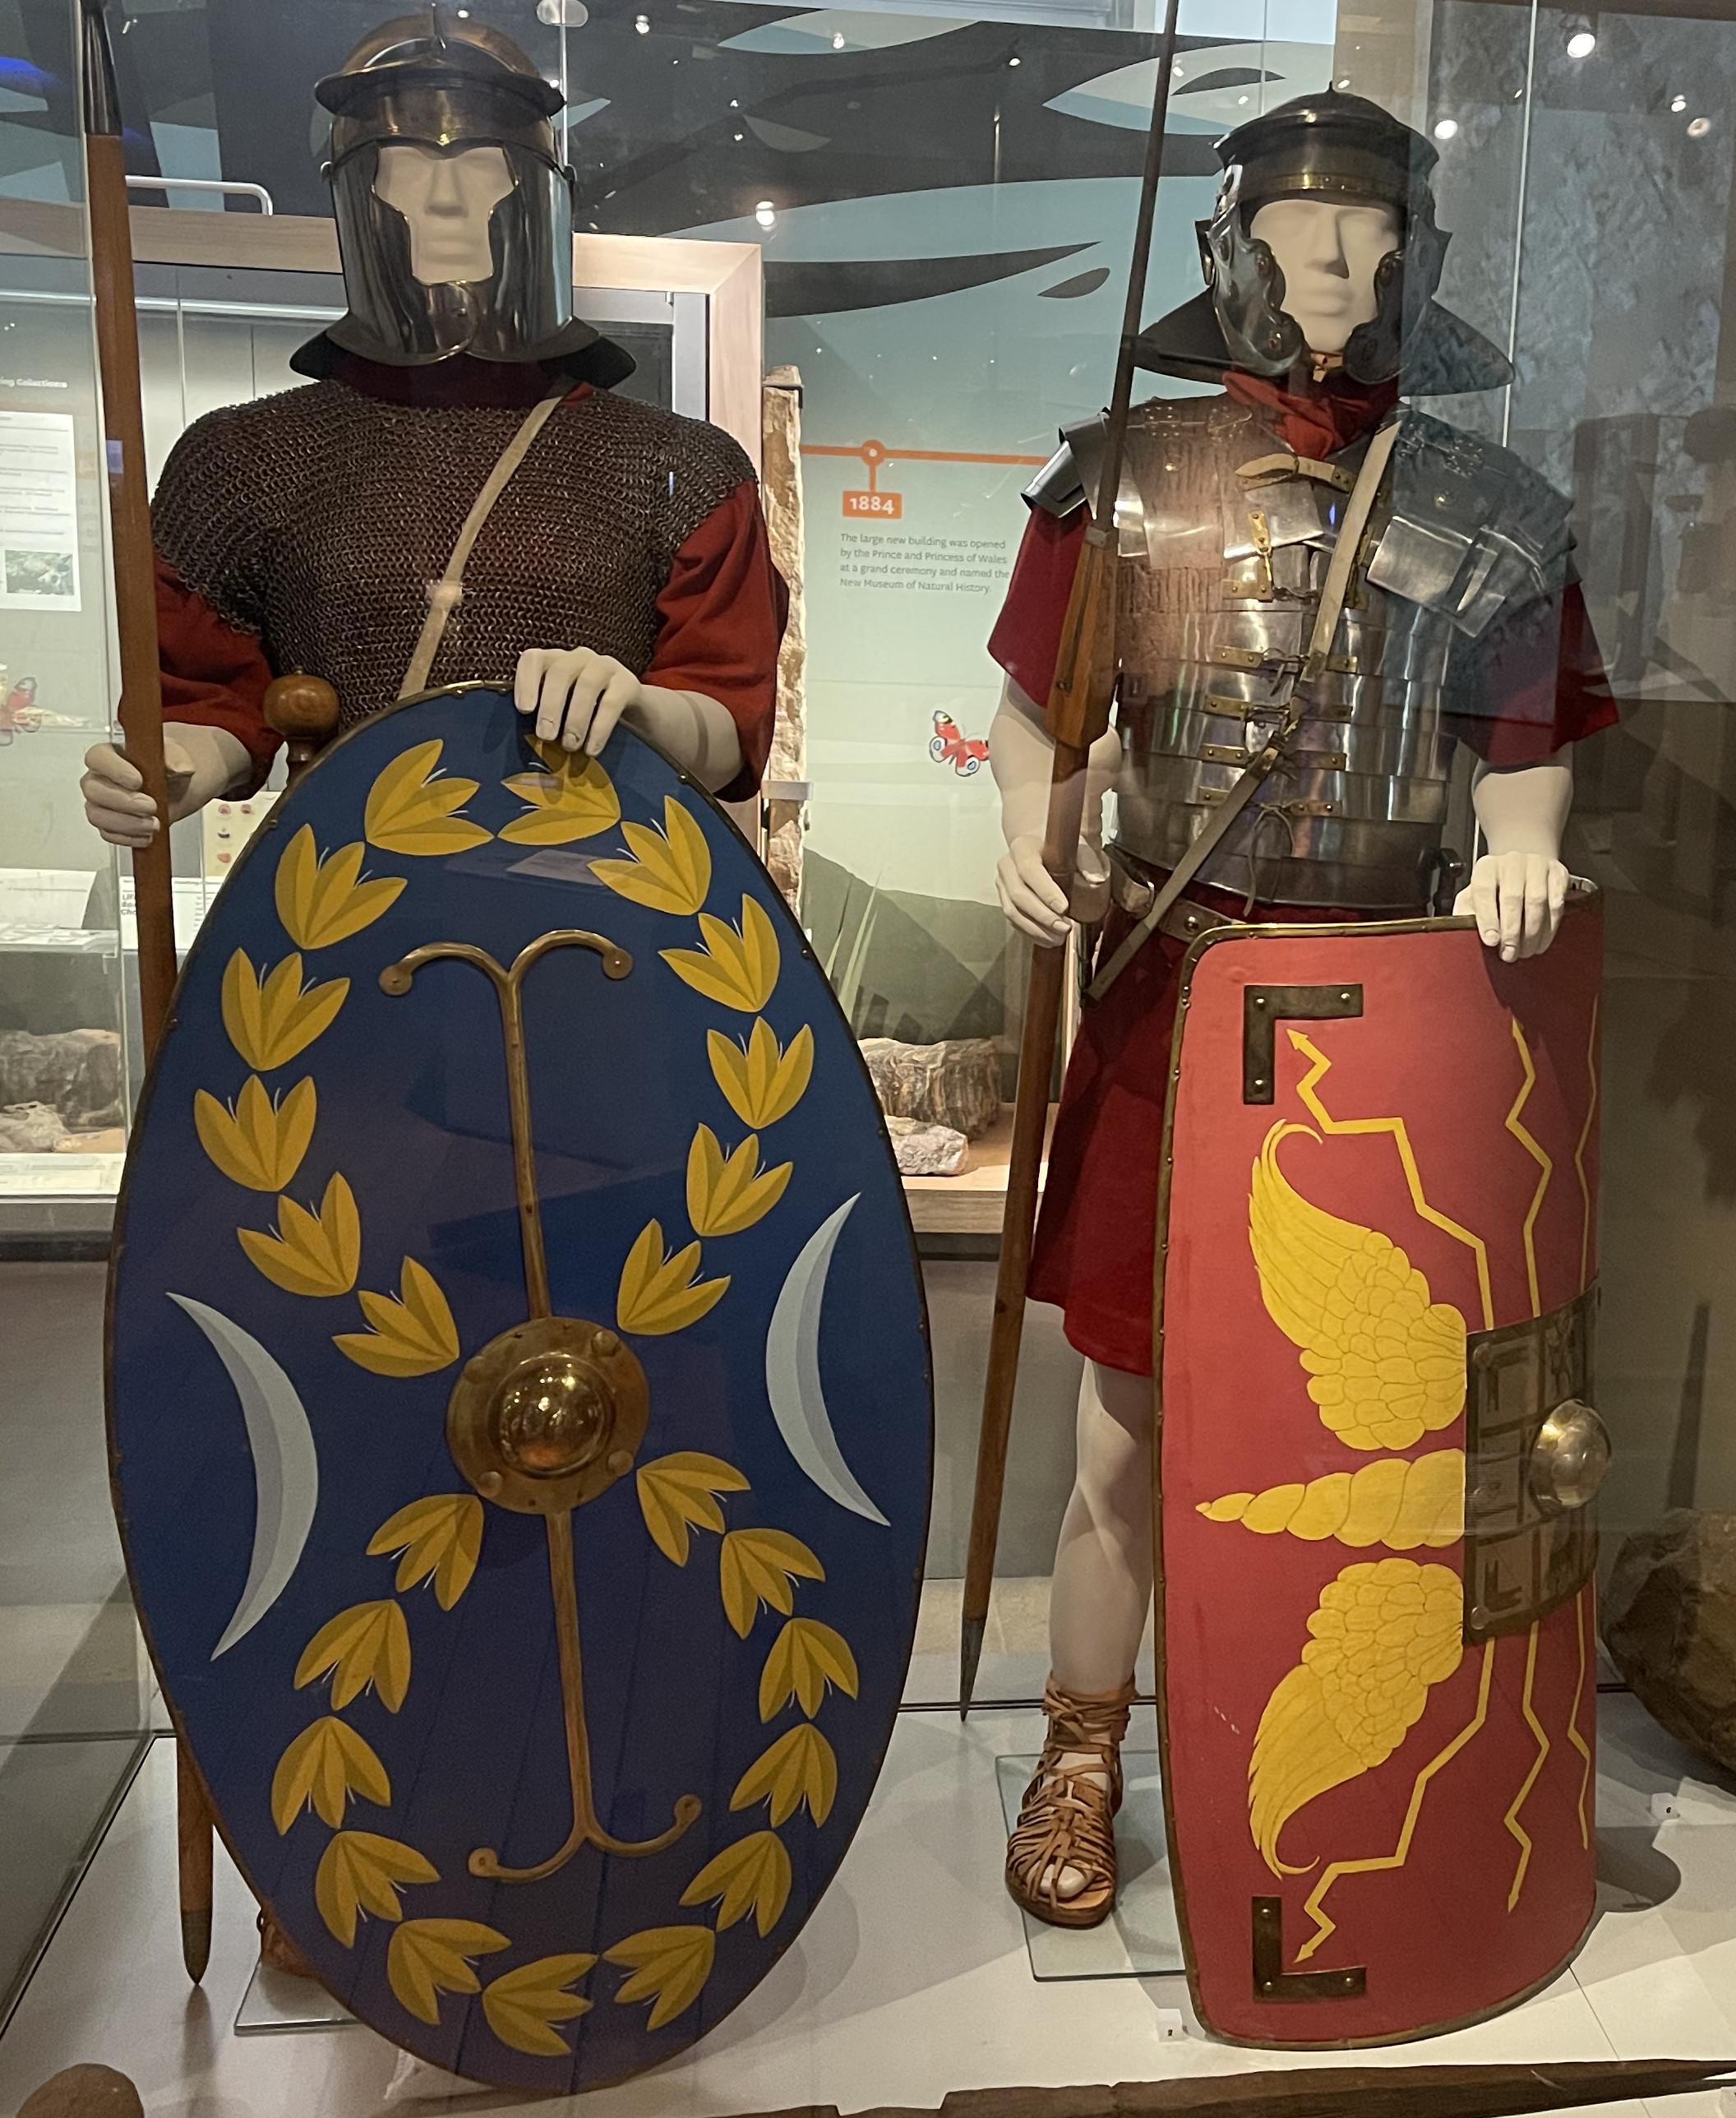
\includegraphics[width=0.8\linewidth]{armour.jpg}
  \caption{\label{fig:armour} A replica of an auxiliary cavalryman's armour
    (left), 2nd century AD. And a roman legionary's (right), late 1st
    century AD.
  Via Hancock Museum}
  \Description{Models Roman auxiliary and legionary with shields and spears.}
\end{figure}

\begin{figure}[h]
  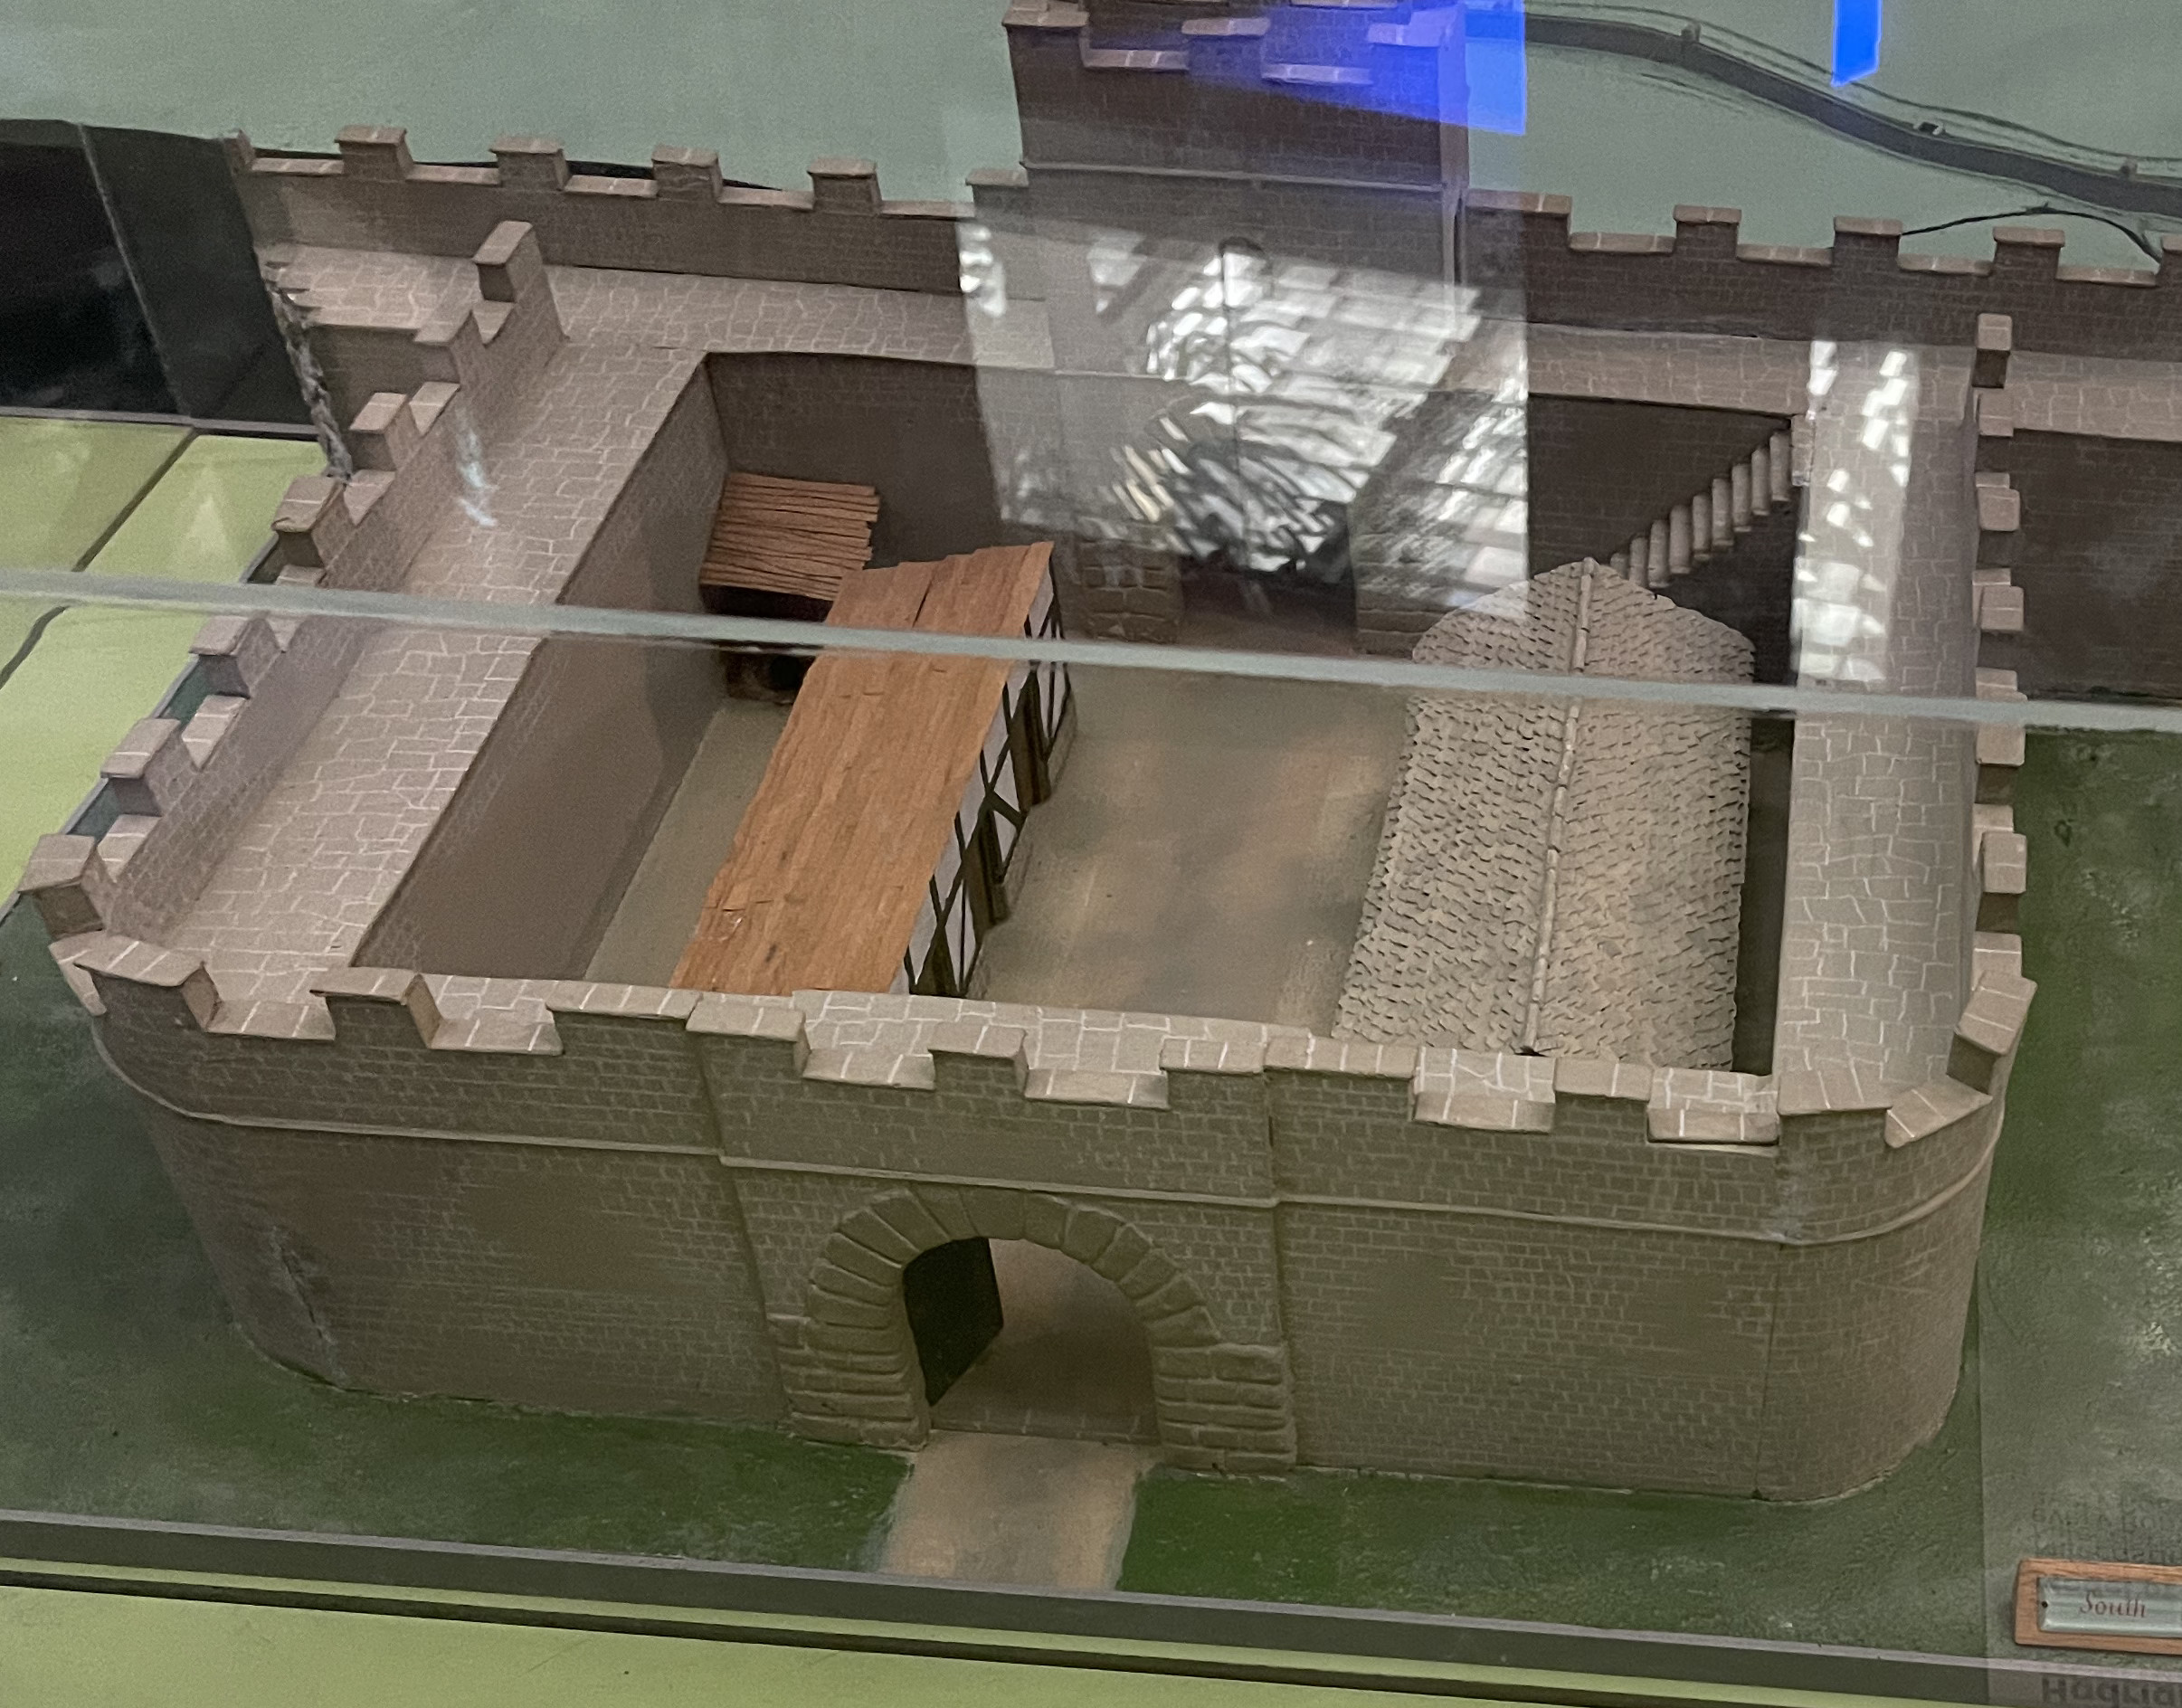
\includegraphics[width=0.8\linewidth]{milecastle.jpg}
  \caption{\label{fig:milecastle}A model of a milecastle from Hadrian's Wall.
  Via Hancock Museum}
  \Description{A scale model of a Roman milecastle from Hadrian's Wall, showing
  a square fortification enclosing buildings and a gate.}
\end{figure}

\begin{figure}[h]
  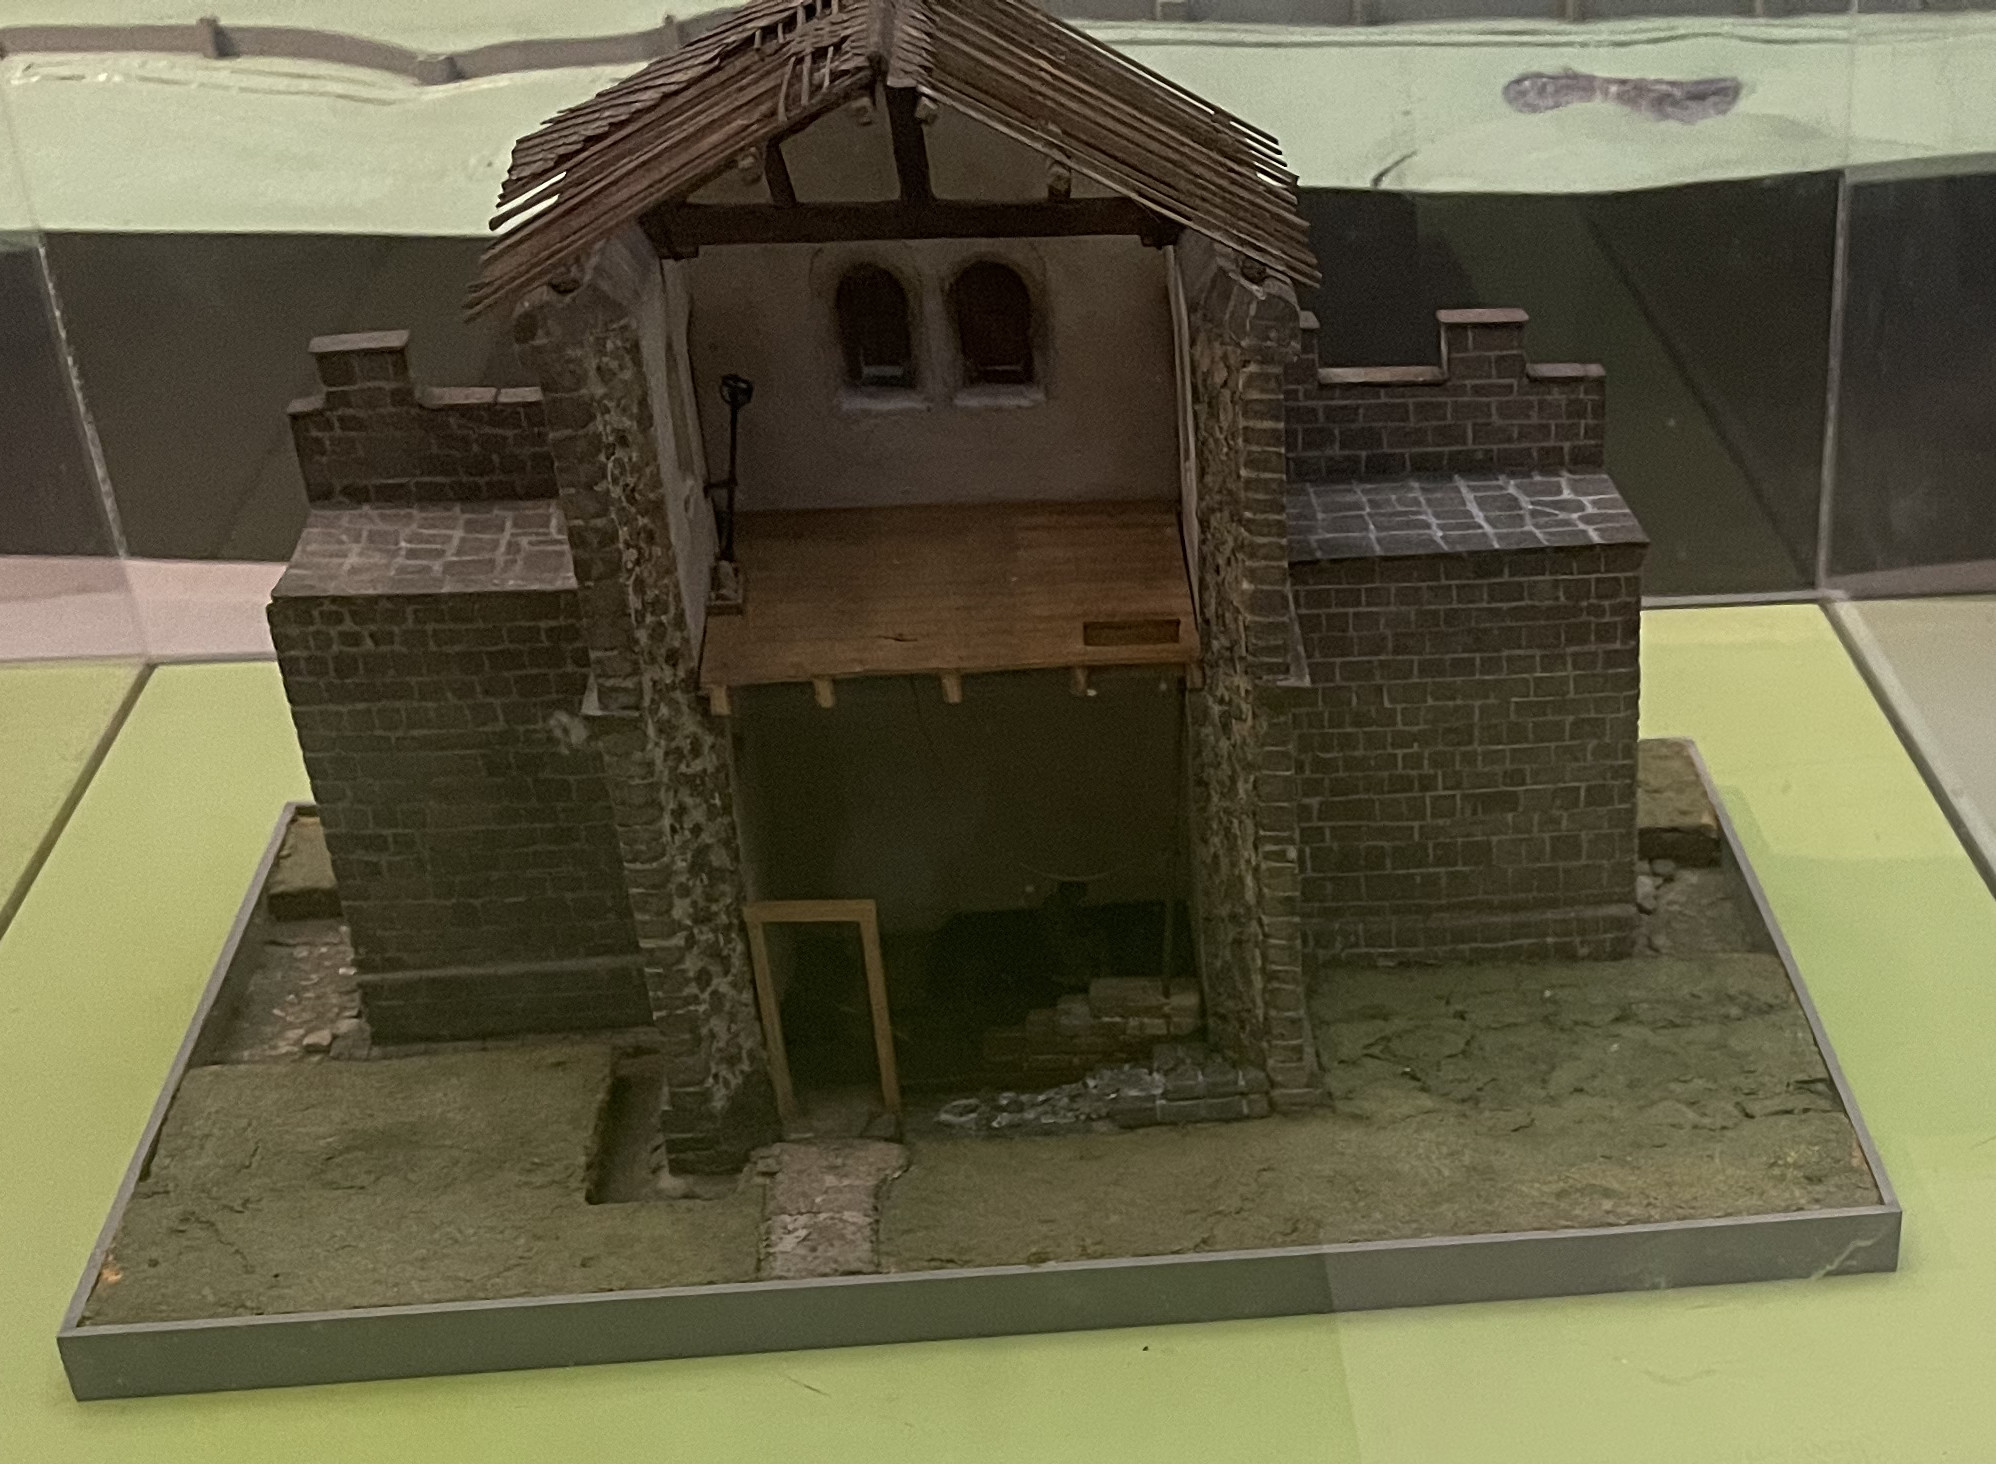
\includegraphics[width=0.8\linewidth]{turret.jpg}
  \caption{\label{fig:turret}A model of a turret from Hadrian's Wall. Via
  Hancock Museum}
  \Description{A scale model of a Roman turret from Hadrians wall, showing a
  cutout of the interior with arrow slits on the top floor.}
\end{figure}

\subsubsection{Literature}
% TODO: Literature}

\subsubsection{A Day in The Life}
% TODO: A Day in The Life at Vindolanda}

\subsection{Technical Research}
% TODO: Technical Research}

\subsubsection{Which Engine?}
% TODO: Which Engine}

Multiple engines were considered, each with their own benefits
and drawbacks as summarised in Table \ref{table:engine_compare}

Virtual reality is a significantly more demanding environment than other games.
While 1080p at 60Hz is a common target for flat screens, VR games must render
two screens at 90-120Hz each, with users often upscaling for enhanced clarity.
Consequently, performance is a crucial requirement for any VR game.
(\hyperref[sec:nfr_performance]{NFR01})

Given the short deadline of the project, industry adoption was also a major
consideration based on the assumption that a more widely adopted engine would
have more resources available to reduce development time. The total number of
games tagged as VR, detected as using a specific engine by
SteamDB (\url{https://steamdb.info/tech/}), and released
after May 2023 (to include current trends) were used to determine adoption.
This methodology has its limitations: by only using SteamDB as a source,
selection bias is introduced as non-steam releases such as itch.io and the Meta
Store are excluded. Additionally, SteamDB's engine detection can produce false
negatives, for example, Godot games can be packaged as a single executable which
will not be detected as shown in Figure \ref{fig:godot_false_negative}. Despite
these limitations, this methodology was considered good enough to get a
high-level overview.

\begin{figure}[h]
  \begin{lstlisting}
    $ ./kicksalot --help
    Godot Engine v4.4 - https://godotengine.org
    ... (output abridged)
  \end{lstlisting}
  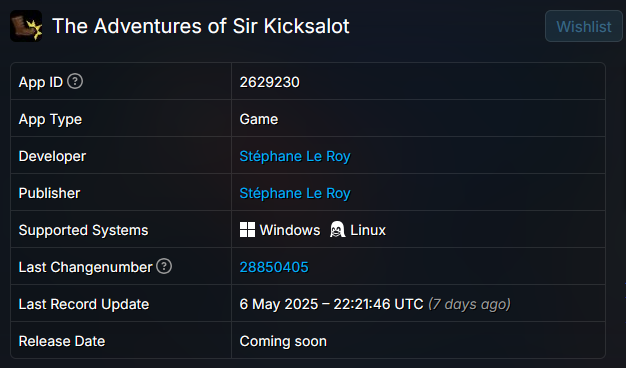
\includegraphics[width=0.8\linewidth]{godot-false-negative.png}
  \caption{\label{fig:godot_false_negative} A game that uses Godot, but is not
    detected as such by SteamDB visible from the lack of a ``Technologies''
  field. https://steamdb.info/app/2629230/}
  \Description{A screenshot of SteamDB's entry for ``The Adventures of Sir
  Kicksalot''}
\end{figure}

A smaller, but important, consideration was the engine's support for Git version
control. While it would have been possible to install and learn Perforce, doing
so would detract from development time, this made Unreal Engine a less practical
choice as it uses binary files for assets, which Git is poorly suited at
versioning.

Based on this analysis, it was determined that Unity best fits the needs of the
game as it is an industry standard and provides a VR template that includes all
locomotion types needed and integration with its UI system. More specifically,
Unity 6.1 was used as it was the latest stable version at time of development.

\begin{table*}
  \caption{The advantages and disadvantages of the considered engines}
  \label{table:engine_compare}
  \begin{tabular}{llll}\toprule
    Feature & Unity & Unreal & Godot \\\midrule

    Language & C\# & Blueprints, C++ & GDScript, C++, C\#, etc. \\
    VR Support & De facto standard & Performance concerns & Yes \\
    Recent Games & $745 (70\%)$ & $351 (30\%)$ & $8 (<1\%)$ \\
    Version Control & Git, text & Perforce, binary & Git, text \\
    Linux Support & Yes & Editor unreliable & Yes \\

    \bottomrule
  \end{tabular}
\end{table*}

\subsubsection{Reference Material}
% TODO: Which other games were referenced as inspiration?}

\paragraph{Virtual Reality}
The implementation of VR in other games, especially with how they handle
locomotion was analysed as inspiration for how it could be handled here. Two
primary methods were identified that would be practical here:

% TODO: Screenshot of options menus in a couple games
\begin{itemize}
  \item Teleport - Player uses the joystick to select a location, then releases
    to teleport. Suggested to inexperienced users.
  \item Smooth - Player holds the joystick to move in a forward direction
    determined by either the headset or controller direction. Suggested to
    experienced users.
\end{itemize}

Given the variety of preferences among users, locomotion types should be
configurable such that allow each user may select what they are most comfortable
with, as well as to add vignette based on their needs. While some games include
more advanced movement such as climbing or jumping, these were not deemed
necessary here.

% TODO: Figure on UI sketch
% TODO: VR inspiration. Mostly in how certain mechanics are implemented}

% TODO: Handling VR: Locomotion}
% TODO: Handling VR: Text}

\paragraph{Other Games}
% TODO: Other games, focus on visual inspiration}

\section{Design \& Implementation}
% TODO: Implementation}

\subsection{The Setting}

While Roman occupation of Britain spanned centuries, it was decided to set this
game during Emperor Hadrian's visit in 122 AD.
\cite[p.176]{danziger_hadrians_2006}, \cite[p.157]{moffat_wall_2009}
This setting gives the opportunity to teach about the rule of Hadrian himself
and the history leading to the construction of Hadrian's Wall, as well as other
events such as the disappearance of the ninth legion circa 120 AD.
% TODO: Source for 9th legion

% TODO: The setting

\subsubsection{The Fort}

% TODO: Page number for fort count, book is in Hancock museum library
During Roman rule, Vindolanda consisted of at least nine forts
\cite{birley_vindolanda_2009} garrisoned by approximately three hundred men and
one centurion, as documented in a report from circa AD 90.
\cite{bowman_military_1991}

\begin{figure}[h]
  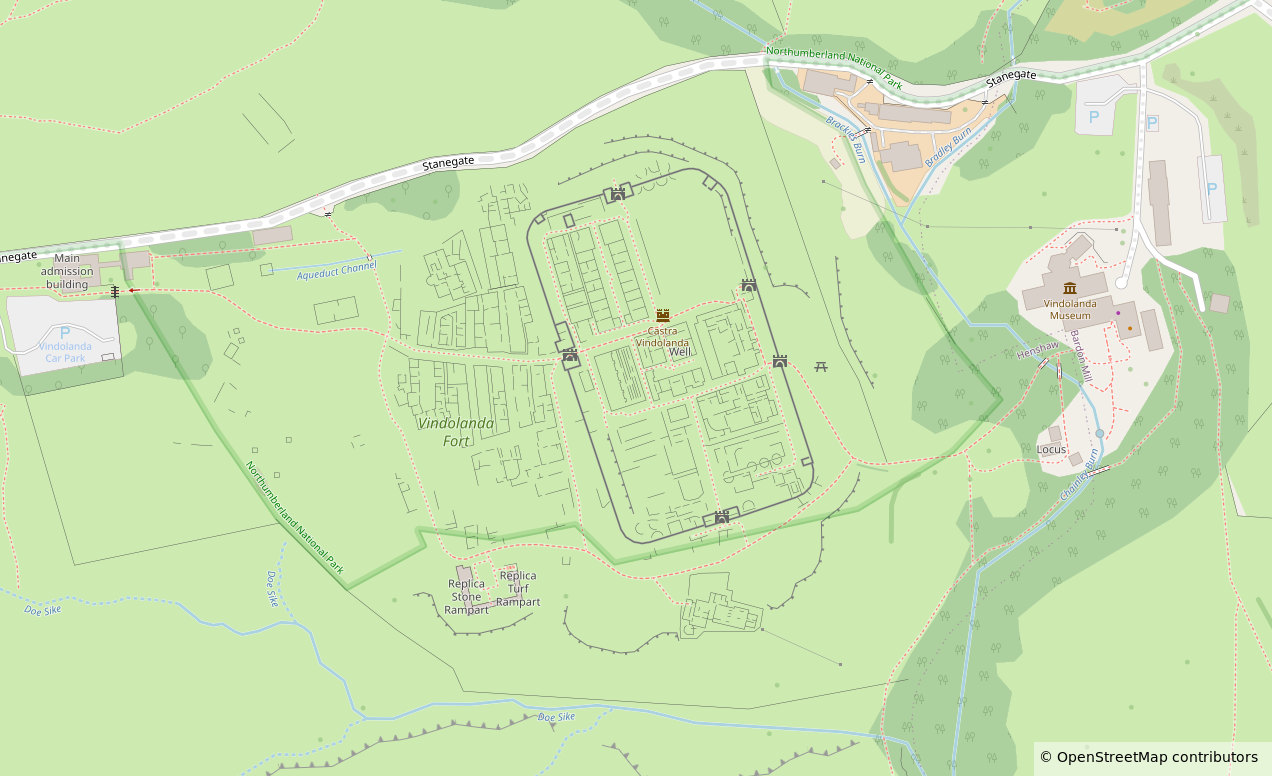
\includegraphics[width=\linewidth]{osm-vindolandra.png}
  \caption{Map of Vindolanda, via OpenStreetMap [ODbL License]}
  \Description{A map of Vindolanda showing the location of interior and exterior
  walls}
\end{figure}

\subsubsection{The Wall}

% TODO: Source for nickname
In addition to the fort, it was also decided to represent Hadrian's wall through
milecastle 39 ``Castle Nick'', situated just over a kilometre north-north-west
where the famous Sycamore Gap tree once stood.

\subsection{VR Considerations}
Virtual reality introduces a unique set of challenges to game development. One
of these is motion sickness, especially for users inexperienced with VR,
\cite{chattha_motion_2020} which is often worsened by smooth locomotion, but can
be mitigated by instead using teleport locomotion, although some users may feel
disoriented after teleporting, the majority find it an easy to use movement
method. \cite{bozgeyikli_point_2016} Due to the target audience of this game
being mostly users without prior VR experience, teleport movement was deemed a
higher priority than smooth movement.

\label{sec:text_scale}
Another challenge, especially when using lower resolution headsets, is the
readability of text. Users require relatively large characters of approximately
20-25mm per metre of distance (distance independent millimetre or dmm
\cite{google_for_developers_designing_2017}) to read comfortably on the lower
resolution HTC Vive, \cite{solum_readability_2019} which is the only headset
available to the researcher and limits text to roughly 8 words per line.

% TODO: Mention difficulties in direct testing due to prior experience
% TODO: Could I talk about personal experience? Would need to be clear that it's
% biased by the learning effect: smooth/teleport both ok, but rotation causes
% disorientation

\subsection{Educational Value}
Educational games are a subcategory of ``Serious Games'', which aim to use the
medium of games to teach through entertainment, and have had positive results in
prior studies, although there is limited data for their efficacy in history.
\cite{backlund_educational_2013}
% TODO: Educational Value. What makes a good educational game?

\subsection{Requirement Analysis}
% TODO: Requirement analysis

A requirement analysis using the MoSCoW method (Must-have, Should-have,
Could-have, and Won't-have) was performed to determine functional and
non-functional requirements for the game.

% TODO: Functional requirements}
\subsubsection{Functional requirements}

\paragraph{FR01 Recreate Vindolanda}
The game \textbf{must} include a recreation of Vindolanda during Hadrian's
rule.

\paragraph{FR02 Recreate Hadrian's Wall}
The game \textbf{should} include a recreation of Hadrian's wall during Hadrian's
rule.

\paragraph{FR03 Before and After}
The game \textbf{should} provide past and present representation of locations
with the option to switch between them.

\paragraph{FR04 Teleport Locomotion}
The game \textbf{must} include teleport-based locomotion.

\paragraph{FR05 Smooth Locomotion}
The game \textbf{should} include smooth locomotion.

\paragraph{FR06 Tutorial}
The game \textbf{should} begin with a brief tutorial on how to move around
using the selected locomotion method, and advise them on the motion sickness
they may experience from smooth locomotion.

\subsubsection{Non-functional requirements}

\paragraph{\label{sec:nfr_performance}NFR01 Performance}
The game \textbf{must} maintain 90FPS during typical gameplay.

\paragraph{NFR02 Linux Support}
The game \textbf{could} include native Linux support.

\paragraph{NFR03 Text Legibility}
Text \textbf{must} be displayed using a clear, easily readable font with high
contrast and a size of at least 25mm per metre of viewing distance to ensure
comfortable reading on the widest range of headsets, as discussed in Section
\ref{sec:text_scale}.

\section{Results \& Evaluation}
% TODO: Results and eval

\section{Conclusion \& Future Work}
% TODO: Conclusion and future work

% TODO: Acknowledgments
\begin{acks}

\end{acks}

\section*{Datasets}

Terrain height maps and textures sourced from DEM.Net Elevation API

Generator: DEM Net Elevation API -
\url{https://elevationapi.com}
Mesh reduction: geometry3Sharp (GradientSpace, Ryan Schmidt) BSL 1.0 License -
\url{https://github.com/gradientspace/geometry3Sharp/blob/master/LICENSE}
Digital Elevation Model: SRTM\textunderscore{}GL3 OpenTopography -
\url{https://opentopography.org/}
Imagery: MapBox Satellite -
\url{https://www.mapbox.com}

\bibliographystyle{ACM-Reference-Format}
\bibliography{vindolanda}

\appendix

\end{document}
